\section{Attack Taxonomy}\label{attack}

In this section, we describe the different attack threat models, methodology and adversary assumptions.
In this work, we provide a comprehensive privacy analysis of graph embedding algorithms by proposing node membership inference attacks, graph reconstruction attacks and attribute inference attack.


\subsection{Node Membership Inference Attacks from Output Predictions}


\begin{figure}[!htb]
\centering
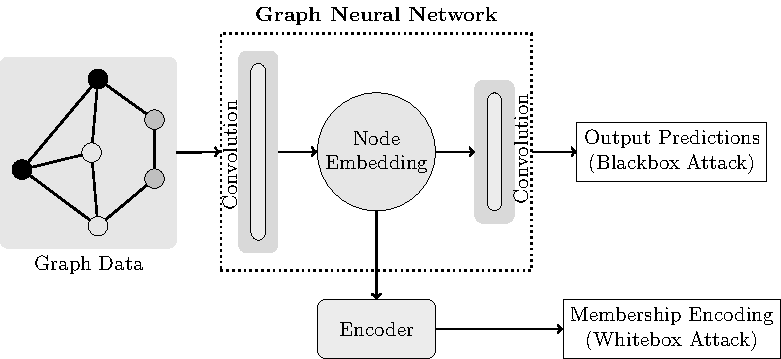
\includegraphics[width=0.85\linewidth]{./figures/Attacks/MIA.pdf}
\caption{To distinguish between members and non-members of $G_{train}$, the blackbox attacks exploit the statistical difference in output predictions while the whitebox attack exploits the intermediate low dimensional feature embedding.}
\label{mia}
\end{figure}

Node Membership Inference attacks allow information leakage in GNNs.
Specifically, the goal of the adversary is to identify whether a user node $x$ is used of not for training the model $f()$.
This is a binary classification problem where the adversary wants to learn the threshold to predict the membership of a user node.
Depending on the adversary's knowledge about $f()$, we consider two settings: blackbox (with and without auxiliary knowledge) and whitebox. %, based on the adversary's knowledge about $f()$.
As shown Figure~ref{mia}, to distinguish between members and non-members the training graph $G_{train}$, the blackbox attacks exploit the statistical difference in output predictions.


\noindent\textbf{Threat Model.} The adversary in a blackbox setting has only access to the model outputs $f(x;W)$ for a given input $x$.
The parameters of the trained model $W$ as well as the intermediate computation are inaccessible to the adversary.
This is a practical setting, typically seen in the case of Machine Learning as a Service, where a trained model is deployed in the cloud and the adversary queries the model through an API and receives corresponding predictions.



\begin{figure}[!htb]
    \centering
    \begin{minipage}[b]{1\linewidth}
    \centering
    \subfigure[Citeseer]{
    \label{fig:nonmem_soft_label}
    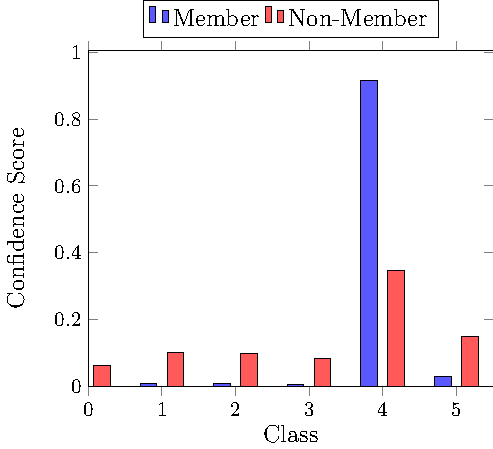
\includegraphics[width=0.5\linewidth]{figures/BBMIA/citeseer_hist.pdf}
    \raisebox{2mm}{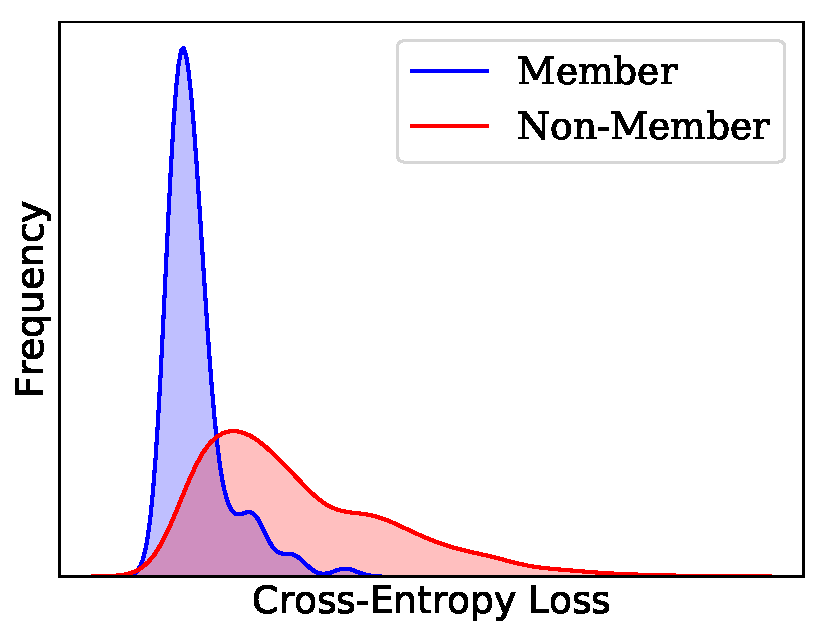
\includegraphics[width=0.5\linewidth]{figures/BBMIA/citeseer.pdf}}
    }

    \subfigure[Cora]{
   	\label{fig:mem_soft_label}
    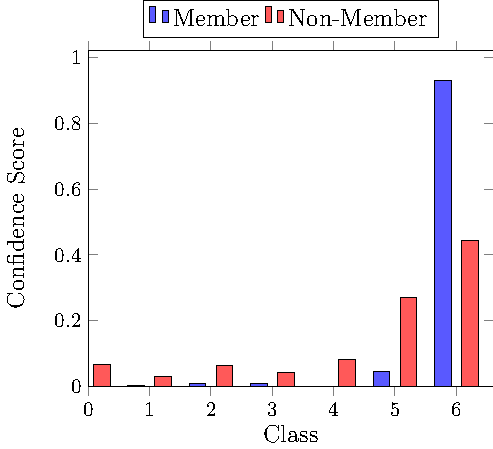
\includegraphics[width=0.5\linewidth]{figures/BBMIA/cora_hist.pdf}
    \raisebox{2mm}{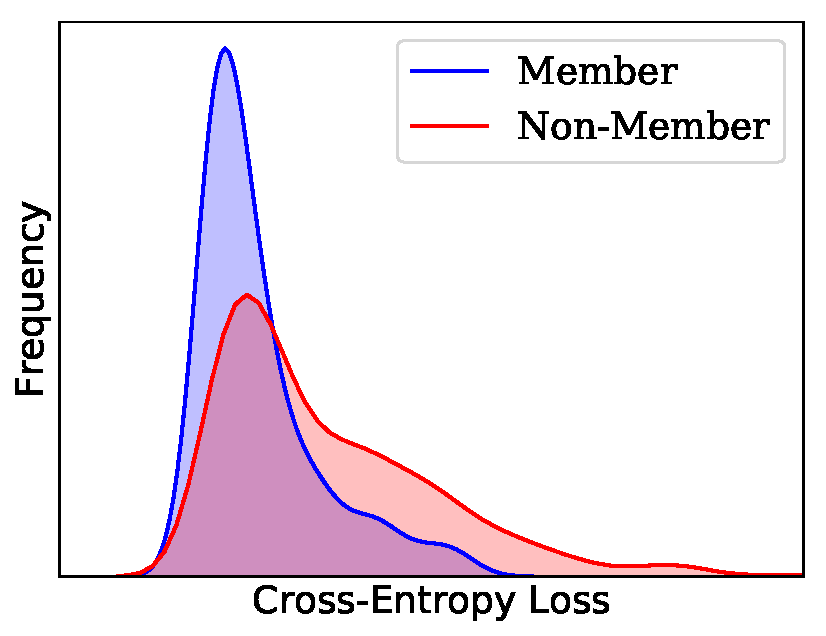
\includegraphics[width=0.5\linewidth]{figures/BBMIA/cora.pdf}}
    }

    \subfigure[Pubmed]{
    \label{fig:mem_soft_label}
    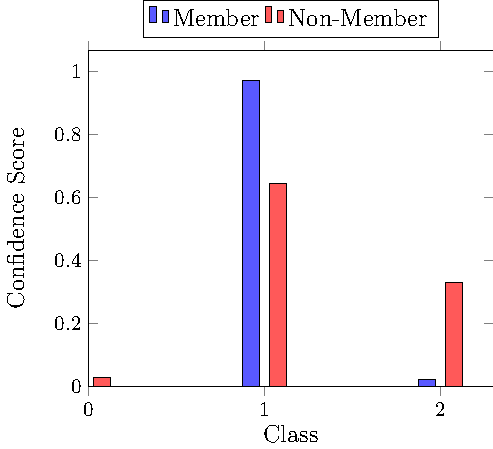
\includegraphics[width=0.5\linewidth]{figures/BBMIA/pubmed_hist.pdf}
    \raisebox{2mm}{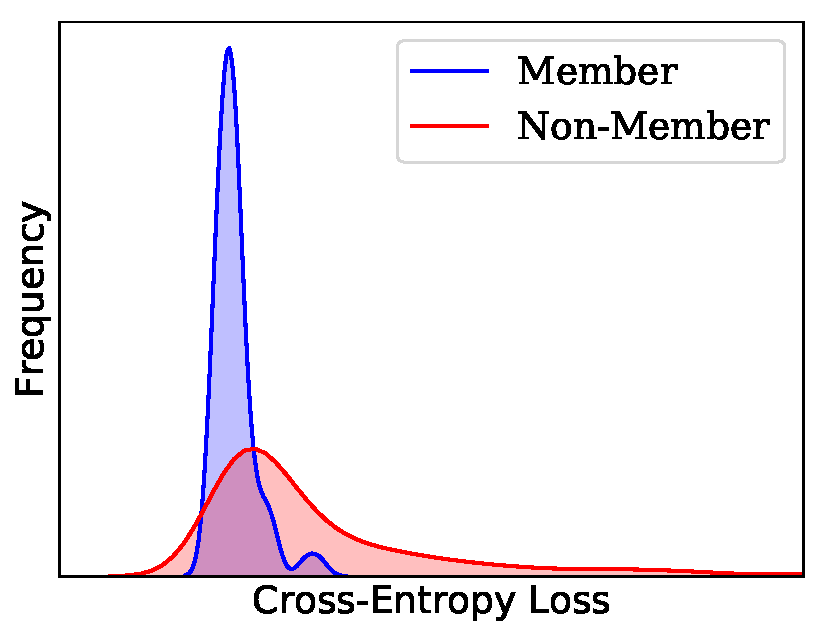
\includegraphics[width=0.5\linewidth]{figures/BBMIA/pubmed.pdf}}
    }
    \end{minipage}
    \caption{Model predictions are more confident for train records compared to test records (left). The extent of overfitting can be detected by a non-overlapping region between the output prediction distributions across all data points (right).}
    \label{fig:NIAcause}
\end{figure}

Blackbox adversary exploits the statistical difference between the confidence in prediction on training and testing data~\cite{7958568}. % add a reference
Figure~\ref{fig:NIAcause} (left) illustrates this difference for models trained on three datasets (details in Section~\ref{setup}) where the prediction confidence for one class is much higher for data points part of the training set.
Predicting with higher confidence on seen $G_{train}$ nodes compared to unseen test nodes is referred as overfitting.
This difference in the output prediction confidence directly results from a distinguishable output distribution between train and test data indicated by non-overlapping region between distributions.
Figure~\ref{fig:NIAcause} (right) illustrates these non-overlapping regions between distributions for the three considered datasets.


Hence, blackbox inference attacks are aimed at exploiting the overfitting aspect of GNNs.
Based on the adversary's auxiliary knowledge about $D_{train}$ distribution, we categorize the attacks into: (a) shadow model attack with auxiliary knowledge of $D_{train}$'s distribution, and (b) confidence score attack with no prior knowledge.

\subsubsection{Adversary with Auxiliary Knowledge (Shadow Attack).} The adversary is assumed to have the knowledge of the underlying data distribution from which the $D_{train}$ was sampled.
This assumption of auxiliary knowledge of underlying distribution is realistic as the data distribution can be collected from real world public datasets available online through social network API's or crawling websites~\cite{logan}.
Further, in this particular work, we assume that the adversary has knowledge about the target GNN architecture which is consistent with prior attack settings~\cite{7958568,logan,10.1504/IJSN.2015.071829,10.1145/3243734.3243834,10.1145/3243734.3243855,10.1145/3319535.3363201}.
However, the attack is transferable across different models~\cite{ndss19salem}.


\begin{figure*}[!htb]
\centering
\resizebox{0.8\textwidth}{!}{
    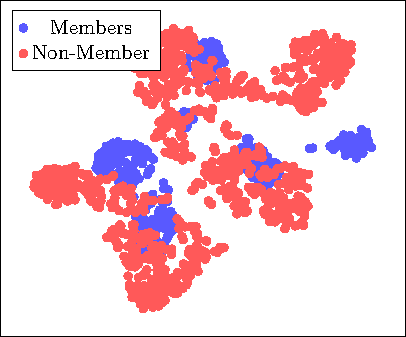
\includegraphics[width=.3\textwidth]{figures/EmbeddingMIA/citeseer.pdf}\hfill
    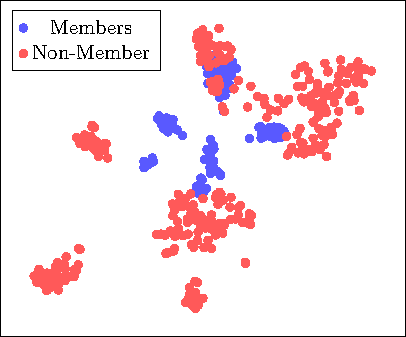
\includegraphics[width=.3\textwidth]{figures/EmbeddingMIA/cora.pdf}\hfill
    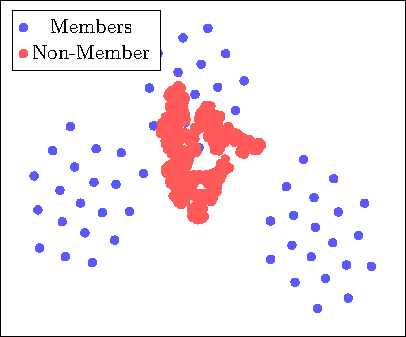
\includegraphics[width=.3\textwidth]{figures/EmbeddingMIA/pubmed.pdf}
  }
    \caption{Whitebox membership inference attacks exploit the distinguishable intermediate feature embedding of train and test records for (a) Citeseer, (b) Cora and (c) Pubmed datasets.}
\end{figure*}

To conduct its attack, the adversary uses her prior knowledge to map the target model's predictions to membership values and hence the attack is supervised.
For a target model $f()$, the adversary trains a substitute model $f_{local}$ on data ($D'$) drawn from the same distribution as $D_{train}$.
The datasets are assumed to be non-overlapping, i.e, $D_{train} \cap D' = \phi$, which makes the attack more practical.
The goal is to train $f_{local}$ to mimic the behaviour of $f()$, i.e, the output predictions should be similar to each other $f_{local}(x;W') \sim f(x;W)$ for the same input $x$ but different parameters $W'$ and $W$ due to training on the different data.
Given the substitute model, the adversary creates a synthetic dataset with binary classes for distinguishing members and non-members (encoded as class 1 and class 0) of $f_{local}$'s training data $D'$ while using the output predictions as the input features.
That is, the synthetic dataset has the input as $f_{local}$'s predictions for an input $x$ classified as "Member" if $x \in D'$ and "Non-Member" otherwise.
In other words, $f_{local}$ is used as a proxy for $f()$ to learn the mapping between the $f()$'s output predictions and the membership information.
The adversary trains a binary attack classifier $f_{attack}$ on the synthetic dataset used to predict whether a new data record was member of $D_{train}$.


\subsubsection{Adversary without Auxiliary Knowledge (Confidence Attack).} In this particular case, we alleviate the data distribution assumption of shadow model making the attack applicable to a wide range of practical scenarios.
Since, the adversary does not have prior knowledge to map the output predictions of target model to classify the membership, the attack is performed in an unsupervised setting.%  and does not use shadow or attack model.

To conduct its attack, the adversary leverages the fact that models with higher output confidence prediction are likely to be members of training data points.
Here, the adversary finds the output prediction with highest confidence and compares whether this is above a certain threshold to decide whether the corresponding input was in the model's training data or not~\cite{8429311,ndss19salem,10.1145/3319535.3354211}.
A large output confidence indicates membership of the data point in the training data.
In order to find the threshold which provides best inference leakage, the adversary sweeps across different values to select the value which best suits the application by looking at the recall.
For instance, if the application requires to obtain a higher precision, the threshold is kept high while for higher recall the threshold is small. We choose our threshold as 0.5.







\subsection{Node Membership Inference Attacks from Graph Embedding}

The adversary in a whitebox setting has access to the model output predictions $f(x; W)$ for an input $x$ as well as the model parameters $W$.
This allows the adversary to compute the intermediate computations after each layer.
This is a strong adversary assumption but practical in cases such as federated learning where the intermediate computations and parameters can be observed~\cite{8835245,DBLP:conf/sp/MelisSCS19}.

%\noindent\textbf{Attack Motivation.}
As explained Section~\ref{graphnn}, GNNs compute the low dimensional feature embedding for the input graph data.
The parameters of the embedding function are updated in each iteration of training and tuned specifically for high performance on the train data resulting in a distinguishable footprint between feature embedding of train and test data points.
Figure~\ref{embedding} illustrates this rationale by plotting feature embedding of train and test records for the three datasets after a dimension reduction using 2D-TSNE algorithm~\cite{vanDerMaaten2008}.



%\noindent\textbf{Attack Methodology.}
The attack is unsupervised since we assume the adversary has no prior knowledge to map the intermediate feature embeddings to a membership value. % (available as auxiliary knowledge in shadow model).
The adversary trains an encoder-decoder network in unsupervised fashion to map the intermediate embedding to a single membership value.
For an input $x$, encoder $f_{enc}()$ generates a scalar membership value which is passed to decoder $f_{dec}(f_{enc}(x))$ to obtain $x$ by minmizing reconstruction loss: $||x - f_{dec}(f_{enc}(x))||_2^2$.
Given the membership values for different training and testing data points, K-Means clustering is used to cluster the nodes into two classes (members and non-members).
For any new input, the adversary can then use this clustering to map it as members or non-members of the training data.
This novel whitebox attack exploits the difference in embedding representation between members and non-members of training data which is not possible for Deep Neural Networks trained on euclidean data where the intermediate activations are abstract (generalize well) and cannot be used to distinguish members and non-members~\cite{8835245}.









\subsection{Graph Reconstruction Attack}

\begin{figure}[!htb]
    \centering
    \begin{minipage}[b]{1\linewidth}
    \centering

    \subfigure[Output Distribution for all records]{
   	\label{fig:mem_soft_label}
    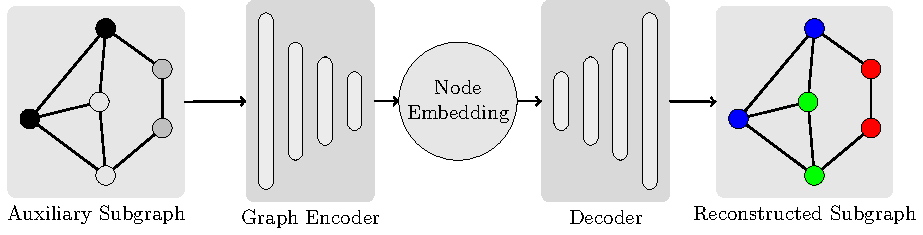
\includegraphics[width=\linewidth]{./figures/Attacks/reconstruction.pdf}
    }

    \subfigure[Output Distribution for all records]{
    \label{fig:mem_soft_label}
    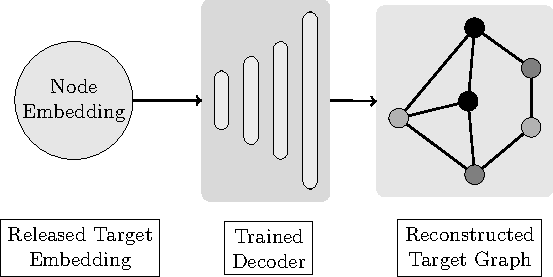
\includegraphics[width=0.6\linewidth]{./figures/Attacks/reconstruction2.pdf}
    }
    \end{minipage}
    \caption{Distribution of the confidence score vectors of the target classifier on the training data and test data of class 29 in the Purchase100 dataset. Each color represents one data record.}
    \label{fig:recattack}
\end{figure}

Adversary Goal


Attack Methodology

\textbf{Link Inference Attack}

Link Inference attacks is a binary classification problem where the adversary aims to infer whether there exists a links between two nodes in the graph.
This translates to identifying whether two people know each other in case of online social networks and identifying the friendship circle which can violate the privacy of the individual.
Link Inference attacks naturally follow from the reconstruction attack where given the reconstructed graph, the adversary can check for an edge between two users using the adjacency matrix.
Write link inference as checking the adjacency matrix...


\subsection{Attribute Inference Attack}

Given an embedding of the graph node $\Psi$

Adversary Goal

Attack Methodology
